\subsection{Operation history and machine layout}

%% ================================= history ==============================
\textbf{Operation history}

LHC \cite{Bruning:2004ej, Buning:2004wk, Benedikt:2004wm, Evans_2008} 
is a two-ring-superconducting-hadron accelerator and collider lies in a tunnel 27 kilometres in circumference and as deep as 175 metres.
It's designed to provide proton-proton (pp) collisions at the center-of-mass energy ($\sqrt{s}$) up to 14 TeV
with a unprecedented luminosity of $10^{34} cm^{-2} s^{-1}$.
In the meantime, it can also collide heavy (Pb) ions with an energy of 2.8 TeV per nucleon and a peak luminosity of $10^{27} cm^{-2} s^{-1}$.
Table~\ref{tab:LHC_parameters} shows the main design parameters of LHC for proton-proton collisions.
\begin{table}[htbp]
  \centering
  \caption{Summary of design parameters of LHC for pp collisions.}
  \label{tab:LHC_parameters}
  \begin{tabular}{cc}
    \hline
    Circumference	& 26.7 km\\
    Beam energy at collision	& 7 TeV\\
    Beam energy at injection	& 0.45 TeV \\
    Dipole field at 7 TeV	& 8.33 T \\
    Luminosity		& $10^{34} cm^{-2} s^{-1}$ \\
    Beam current	& 0.56 A \\
    Protons per bunch	& $1.1 \times 10^{11}$ \\
    Number of bunches	& 2808 \\
    Nominal bunch spacing	& 24.95 ns \\
    Normalized emittance	& 3.75 $\mu$m \\
    Total crossing angle	& 300 $\mu$rad \\
    Energy loss per turn	& 6.7 keV \\
    Critical synchrotron energy	& 44.1 eV \\
    Radiated power per beam	& 3.8 kW \\
    Stored energy per beam	& 350 MJ \\
    Stored energy in magnets	& 11 GJ \\
    Operating temperature	& 1.9 K \\
    \hline
  \end{tabular}
\end{table}

LHC was built from 1998 to 2008. 
It started its first beam in September 2018, but then was interrupted by a quench incident only after a few days running.
Then it resumed the operation in November 2019 with a low energy beams.
From March 2010, physics runs took place at the energy of 7 TeV,
Later on, this energy was increased in 2012 to $\sqrt{s} = 8TeV$, with an integrated luminosity of 20.3 $fb^{-1}$,
and this period is called “Run-1”.
After run-1, the LHC was shut down for two years for hardware maintenance and upgrade, starting from February 2013.

The second operation period with higher center-of-mass energy at 13 TeV started from 2015 called "run-2".
And it continued to the end of 2018 with total integrated luminosity reaching about 147 $fb^{-1}$ for ATLAS.
Figure~\ref{fig:lumi_vs_month} (left) shows the cumulative luminosity versus month delivered to ATLAS during stable beams 
at each years from 2011 to 2018,
while the right one shows luminosity versus time delivered to ATLAS (green), recorded by ATLAS (yellow), and certified to be good quality data (blue) 
during run-2 pp collisions.
\begin{figure}[!htb]
  \centering
  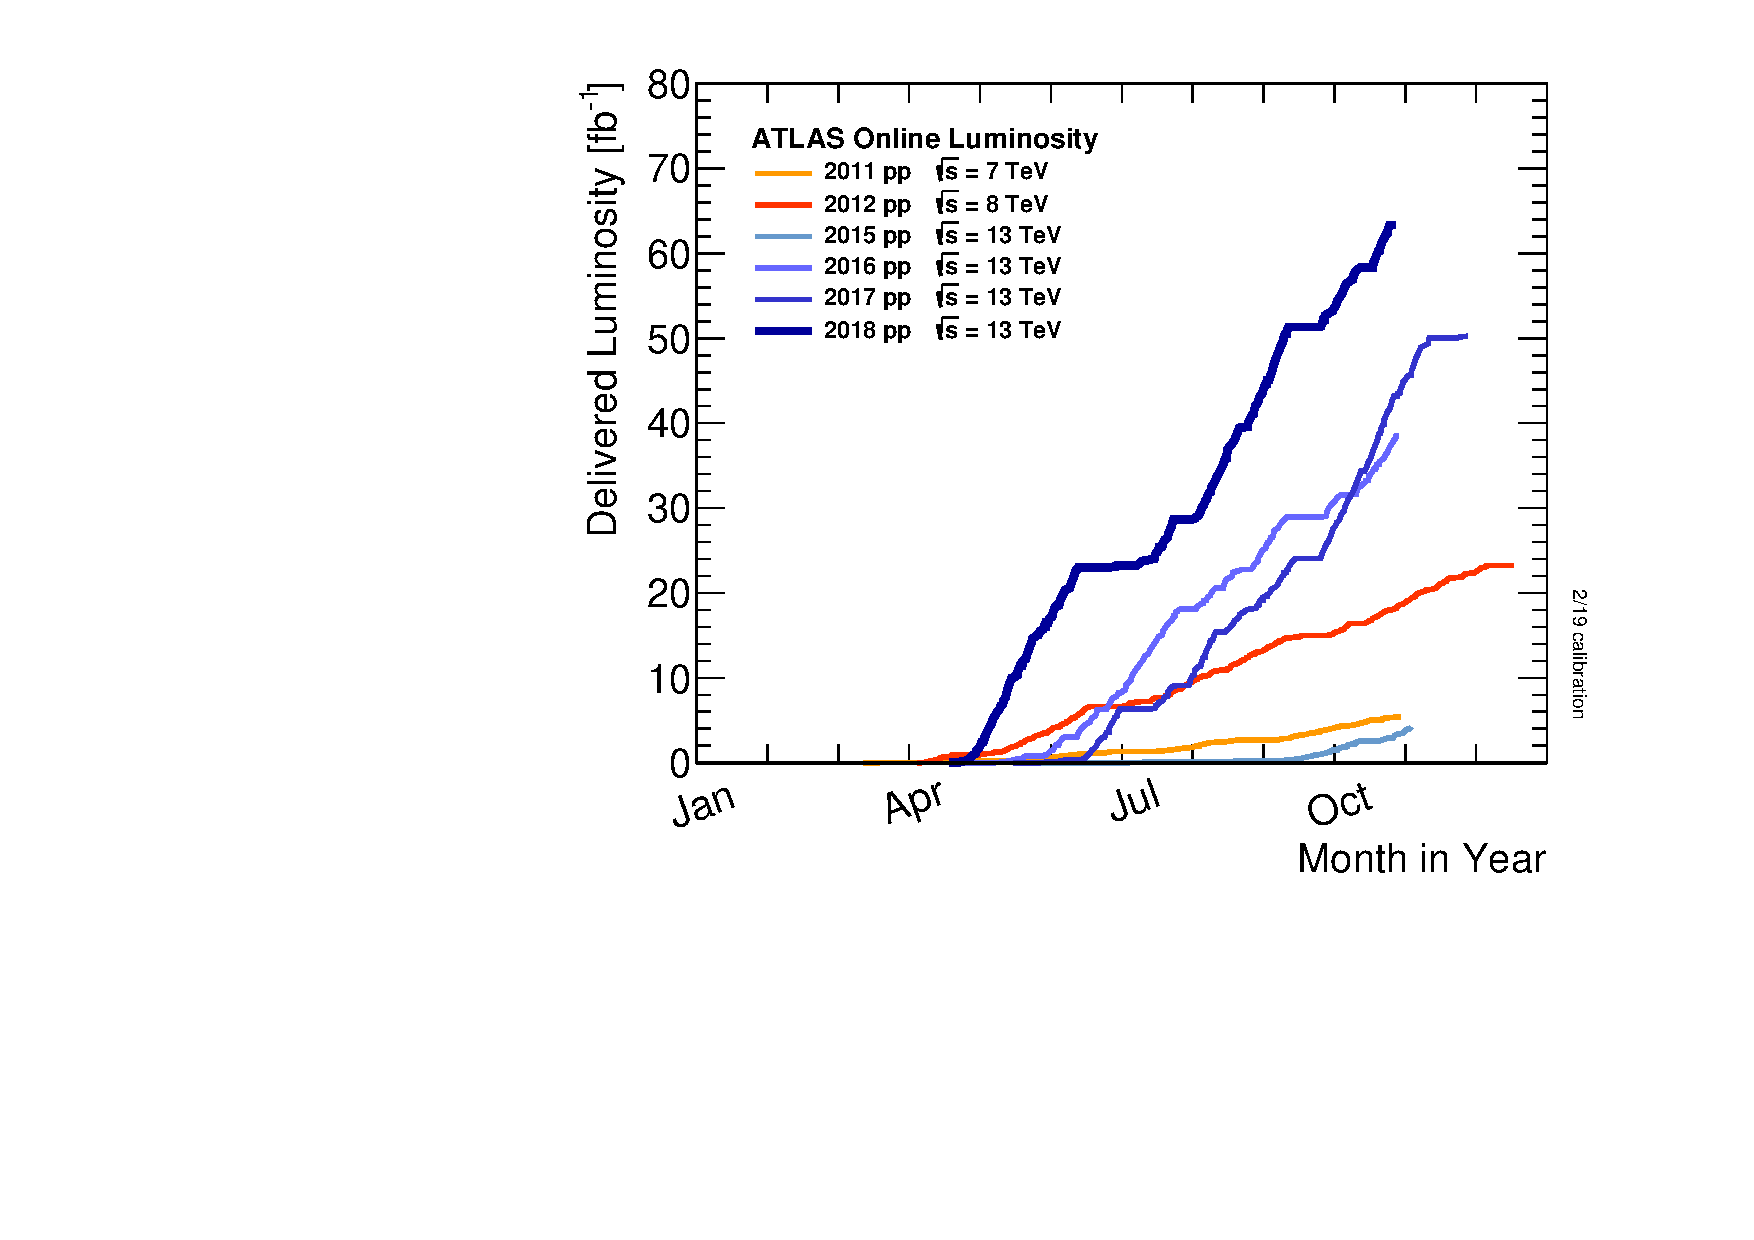
\includegraphics[width=0.48\textwidth]{figures/Detector/intlumivsyear.pdf}
  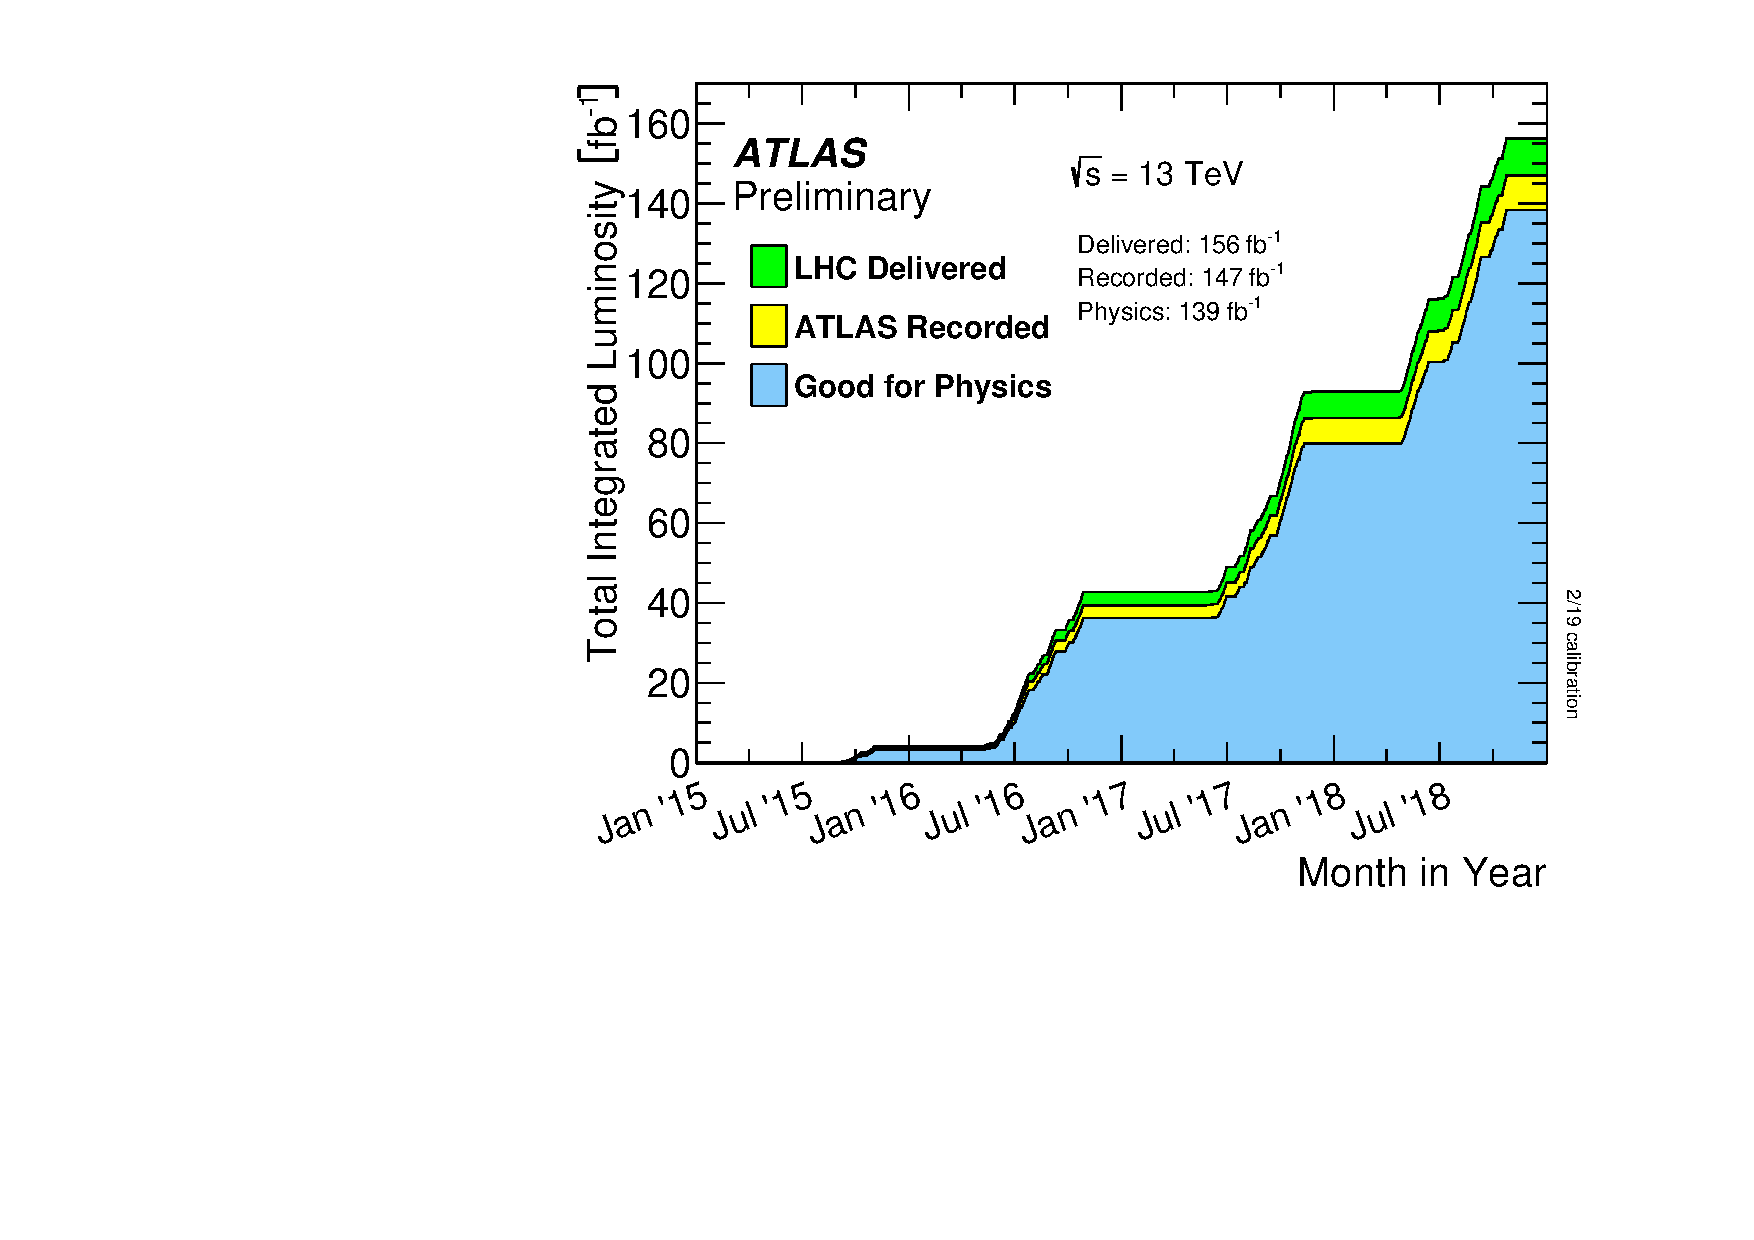
\includegraphics[width=0.48\textwidth]{figures/Detector/intlumivstimeRun2DQall.pdf}
  \caption{Cumulative luminosity versus time in ATLAS.}
  \label{fig:lumi_vs_month}
\end{figure}

%% ======================================= layout ==============================
\textbf{Machine layout}


